
In this chapter we shall discuss the programming techniques, language characteristics and APIs
used in implementing each system component and algorithm. We shall highlight the APIs used and the 
integration with the Eclipse platform, as well as how OOP techniques and patterns are used to implement 
some of the algorithm presented in chapter \ref{Algorithm Design}.

\section{Eclipse platform and Draw 2D graphics API}

The Eclipse platform is an open source, cross-platform IDE(Integrated Development Environment) environment 
developed and maintained mainly by a consortium which includes companies such as IBM, Red Hat and SuSE. 
It mainly targets Java developers, but it also supports the plug-in additions to extend its functionalities 
for various programming languages. It can also work with typesetting languages such as LaTeX and be integrated 
with revision control systems like CVS(Concurrent Versions System) and GIT.

Eclipse has become popular amongst both software and hardware developers. Its main advantages are: faster 
code navigation and visualisation, better code understanding through tracing, referencing and hierarchical 
display functionalities and resource usage management and monitorization. The platform is also able to 
handle makefile generation, compilation and, most importantly, integration with debugging and profiling tools.

This IDE enviroment has been chosen mainly because of it can operate cross-platform and it is open source. 
Moreover, the code does not have to be written and organized differently in order to function on different 
platforms, such as Windows or OS-X. The drawbacks are also relevant, since running any application requires 
the entire platform to load, which is significantly more taxing on resources than a command line application 
would be. Thus, the IDE can be considered suboptimal from this perspective if the user is not fully interested 
in all of its capabilities.

Since it is an open source project, the Eclipse platform offers developers various APIs to facilitate and 
encourage the community to extend or improve existing functionality or add new capabilities. One such 
API is the Draw-2D graphics library, which is an extension of the SWT library. This library is generally used 
to implement small widgets which handle the drawing of charts and diagrams.

By default, the API can render any object which the SWT library can handle. In addition, it adds a series of 
classes and methods which allow the user control over the position of each object, its contents and other 
graphical characteristics such as colour and style. We shall continue by enumerating and discussing some of 
the main Draw-2D classes used in the implementation.

\subsection{Draw 2D Point class}

Points represent the basic operating unit of the library. They do not refer to a graphical entity, but a 
spatial one. They are used to define the location (coordinates) of a figure or shape, designate an axis 
or segment or define the corners of a polygon when placed in an ordered list.

The class exposes API for accessing and manipulating coordinates, as well as basic mathematical computations 
such as transposing points and calculating the euclidian distance between two points. Still, the API lacked more 
advanced computations such as: manhattan distance, determining the angle between the X axis and the line 
designated by two points and moving the point in a general direction with a given speed. These functions 
have been implemented and are shown below:

\begin{lstlisting}[caption={Functions added for the Point class}, language=Java]
public int manhattanDistance(Point p1, Point p2) {
	return Math.abs(p1.x - p2.x) + Math.abs(p1.y - p2.y);
} 

public double computeAngle(Point p1, Point p2) {
	int deltaY = p1.y - p2.y;
	int deltaX = p1.x - p2.x;
	return (Math.atan2(deltaY, deltaX) * 180) / Math.PI;
}

public void movePointInDirection(Point p, double speed_factor) {
	p.x += speed_factor * (int) Math.cos(angle);
	p.y += speed_factor * (int) Math.sin(angle);
}

\end{lstlisting}

\subsection{Draw 2D Rectangle class}

The rectangle in the Draw 2D library does not simply stand for the geometric shape. When drawn, every 
figure and component placed on the canvas is placed in an enclosing rectangle which delimits its size 
and relative position by means of five points: the center and four corners. 

Whenever testing for collisions, it is not the figures and shapes which are intersected, but rather their 
enclosing rectangles. This allows for a certain margin of error to be taken into account. More so, when 
testing for collisions, the \emph{intersect()} method of the Rectangle class returns a new Rectangle 
representing the collision area. By doing so, it facilitates the correction step, since the algorithm 
knows exactly how much each figure must be moved.

\begin{figure}[ht] \centering
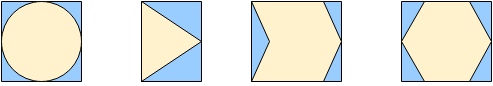
\includegraphics[width=0.75\textwidth]{img/implementation/rectangles.png}
\caption{Geometric figures and their bounding rectangle} \end{figure}

\subsection{Figure and PolylineConnection classes}

Figures are the main units drawn on the canvas by the graphical renderer. A figure can 
range from the simple outline of a geometrical shape to complex elements which can hold labels (titles), text 
or even other figures. Custom figures may even be modeled as icons or pictograms, since their background can be 
coloured, their borders can be stylized and by using extended API even animations could be created.

Polyline connections are wrapper classes which essentially hold a list of points. These points are used to create 
lines or paths. This is achieved by using the inner list of points to draw Rectangles of negligible height. Just 
as figures, these lines can be stylized and, in case of representations of directed connections, they can be 
decorated to emphasize these directions.

The implementation extends both of these classes in order to implement graphical elements with user oriented 
functionalities. First, the Figure class is extended by the NodeFigure and ModuleFigure classes. A NodeFigure 
is a figure used when drawing a simple graph for which the user does not provide any special information.
It holds and displays only the name of a node. The ModuleFigure, on the other hand, is used to represent a 
module as it is seen from a HDL designer point of view. It holds information regarding ports, their direction 
and where they are connected. This type of figure contains and displays labels and text elements which the user 
can interact with.

PolylineConnection is extended as a OrthogonalConnection. This special type of connection holds references to the 
figures which it connects and implements a listener. The role of the listener is to watch for modifications made 
to the position of the figures. Whenever one changes, the OrthogonalConnections announces the router that it 
must be recalculated. If an obstacle has been placed on the path in the meantime, the new path shall be computed 
to go around it.

\section{Modules implementation}

The modules which compose the application, as listed in chapter \ref{System Architecture}, utilize a set of Java 
and OOP concepts and patterns. In this section we shall discuss some of these notable patterns.

\subsection{Input file format}

As was previously presented, the input graphs are read from files written in a certain format, akin to a programming 
language. This facilitates data manipulation and enables the user to easily describe and understand the model. 

The structure of such a file is shown below:

\begin{lstlisting}[caption=Input file example]

begin graph
    name: Example Graph
        begin node
            name: A
            id: 1
            connections: B
        end node
        begin node
            name: B
            id: 2
            connections: A,C
        node end
        gebin node
            name: c
            id: 3
            connections: A,D
        node end
       	begin node
            name: D
            id: 4
            connections: C
        node end
end graph

\end{lstlisting}

\subsection{Parser implementation}

The input files parser is implemented using exclusively Java file oriented API. Files are read using a Scanner object, 
which allows the reading of bytes from the file until certain specified characters are encountered. Upon reaching 
such a character, the scanner provides a String object containing the read data. 

Next, a StringTokenizer splits the String into tokens. Rules and patterns (of the grammar) are applied on these tokens 
to determine wether they form valid expressions and provide useful information.

\subsection{Graph data and elements}

The graph object itself is constructed using the Factory pattern. Nodes and Edges are both implementations of a 
GraphElement interface. The graph keeps a list of GraphElement objects which is populate by the parser as the input 
files are decoded. In order to differentiate between each type of element, the interface exposes the method 
\emph{getType()}. Each object returns a different value of an enumeration called ElementType. 

Using this pattern, the graph object does not have to keep two individual lists, one for each type of element. This 
helps keep the memory usage lower in case of large amounts of data. When another module requires all elements of a 
certain type, a new list is constructed on the fly and passed to the caller.

\begin{lstlisting}[caption=Basic class structure for factory implementation, language=Java]
public interface GraphElement {
	public ElementType getType();
}

public enum ElementType {
	VERTEX, EDGE;
}

public class Vertex implements GraphElement {
	@Override
	public ElementType getType() { return ElementType.VERTEX;}
}

public class Edge implements GraphElement {
	@Override
	public ElementType getType() { return ElementType.EDGE;}
}

public class Graph {
	public List<GraphElement> elements;
	...
	public List<GraphElement> getElementsOfType(ElementType type) {
		List<GraphElement> result = new ArrayList<GraphElement>();
		for (GraphElement ge : elements) {
			if (ge.getType.equals(type)
				result.add(ge);
		}
		return result;
	}
}

public class Parser {
	...
	public void parse(File inputFile) {
		...
		graph.elements.add(createElement(parsedData));
		...
	}
	...
}

\end{lstlisting}

\subsection{Graph processing modules}

The modules which utilize graph data and perform modifications on it: planarity tester, layout processor and edge router 
have at their core consecrated algorithms. Certain modifications are made to these algorithms in order to properly integrate 
them in the Java environment. Also, in some cases, elements from different classes of algorithms are combined in the 
implementation (for example the rule-based placing algorithm).

The planarity tester is a direct implementation of theorems 1 and 2 presented in the Algorithm Design chapter. However, there 
is also an implementation of Chiba and Nishizieki's algorithm which is used to confirm planarity. This algorithm is called 
when the necessary condition specified by the theorems holds.

In the case of layout processing, the grid type layout algorithm uses an implementation of the white path theorem algorithm 
based on DFS(depth first search) to construct the spanning tree used to layout the algorithm. The pseudocode of the white path 
theorem algorithm is listed below:

\begin{lstlisting}[caption=Spanning tree algorithm using DFS]
PROCEDURE SPANNING-TREE {
BEGIN
	choose arbitrary vertex v;
	addToSpanningTree(v);
	WHILE (unvisited vertices)
	BEGIN
		IF (v has unvisited neighbours)
		BEGIN
			u = chooseNeighbour();
			markAsVisited(u);
			addToSpanningTree(edge(v,u));
		END
	END
END
\end{lstlisting}

The rule-based layout processor and the edge connection router are direct Java implementations of the algorithms described 
in the system architecture chapter.

